\chapter{Analyse des besoins}

\section{Besoins fonctionnels}
%mettre le tableau ici
\subsection{Besoins essentiels}

%Hierarchisation: selon les phases du projet %%%%%%%%%%%%

\subsubsection{Importation}

\textbf{• Importer un fichier de données (sous format csv)\\} L'utilisateur choisit parmi sa propre bibliothèque de fichiers un fichier sous format {\tt csv} qui contient des lignes de données sur lesquelles il veut appliquer son code mapReduce. L'extension doit être en .csv mais en revanche nous ne limitons pas la taille du fichier (surtout qu'on est dans un contexte de Big Data). Plus de détails sur le fichier est retrouvé dans le chapitre 4 Implémentation.\\

\textbf{• Importer un fichier contenant les fonctions de mapReduce\\}   
 Donner la main à l'utilisateur pour charger son propre code mapReduce avec les 3 fonctions à implémenter "map", "reduce" et "getPartition". Ce sont ces fonctions qui serviront pour le traitement des données en {\tt csv} qu'il a fournit. Le fichier doit donc être sous format {\tt js} mais par contre il n'est pas nécessaire d'en fournir un.\\

\subsubsection{Configuration} 

\textbf{• Configurer le cluster de map\\ } Offrir la possibilité à l'utilisateur de fournir le nombre de machines ainsi que le nombre de coeurs par machine. Par contre, il est limité par un maximum de 20 machines à 24 coeurs chacune pour des raisons expliquées plus tard dans ce document. \\

\textbf{• Configurer le nombre de Reducer du programme\\}  Il est possible de préciser que le code mapReduce sera traité avec un nombre de tâches de reduce (Reduce Task) bien défini. En effet, la simulation peut varier si on a une seule tâche de reduce, dans ce cas toutes les données seront transférées vers un seul {\tt Slot} et le temps de traitement sera plus long. Par contre, utiliser plusieurs reducers permet une bonne parallélisation selon les cas. Pour ce nombre, il est obligatoire de ne pas dépasser le nombre de slots existants dans la phase de map.  \\

\subsubsection{Modification} 

\textbf{• Modifier les fonctions de mapReduce\\} C'est un besoin étroitement lié à "Importer un fichier contenant les fonctions de mapReduce". Quand l'utilisateur joint son fichier .js, celui-ci est directement chargé dans une zone de texte totalement modifiable. Ainsi, il peut voir son propre code contenu dans le fichier mais aussi effectuer directement des modifications dessus sans avoir à l'ouvrir ailleurs dans un éditeur de texte. C'est une fonctionnalité très utile pour pouvoir tester son code sur plusieurs cas et voir à chaque fois la simulation obtenue.  \\

\subsubsection{Visualisation}

\textbf{•  Visualiser la simulation de l'exécution de mapReduce\\} C'est le service principal offert par notre application. Suivant les entrées de l'utilisateur (données csv, code mapReduce en js et configuration du cluster), un graphique est généré en dessous de la zone de code. Il est affiché alors le process de mapReduce selon ses spécifications.\\

\textbf{• Consulter les résultats sur console\\} En plus du graphique, l'utilisateur peut notamment voir les résultats des variables de sorties des différentes phases. Ce besoin est intéressant quand il veut consulter les résultats des phases de partitioner et de shuffle qui ne sont pas inclus dans la simulation graphique pour ne pas allourdir la lisibilité de ce dernier.\\

\textbf{• Consulter les données exécutées sur un slot\\} Une fois la simulation affichée et le graphique généré, on obtient l'ensemble des machines avec leurs différents coeurs ainsi que les liaisons qui montrent la distribution des données. Pour consulter les données exécutées sur un slot en particulier, l'utilisateur clique sur ce slot. Une zone à droite de la page est alors remplie avec les différentes lignes exécutées sur ce map ou bien reduce (un slot peut contenir soit un map soit un reduce).\\ 
 
\subsubsection{Exportation}

\textbf{• Exporter le résultat de la simulation\\} L'utilisateur peut récupérer les données de sortie du process de mapReduce sous forme d'un fichier de données {\tt csv}. Ce fichier contient toutes les lignes de résultats ayant chacune la structure suivante: "clé; valeur".


\subsection{Besoin optionnel}

\textbf{• Exporter les fonctions générées en langage Java\\} Ceci permet d'avoir le code Java du process MapReduce équivalent à celui en Javascript utilisé pour traiter les données. Ce besoin est facultatif en vue du manque de temps que nous puissions rencontrer.

\subsection{Priorité des besoins fonctionnels}
En plus du découpage besoins essentiels/besoins optionnels, nous pouvons indiquer la priorité des besoins. (Voir tableau ci-dessous)
\begin{center}
\begin{tabularx}{\textwidth}{|X|X|}
  \hline {\bf Besoins} & {\bf Priorité attribuée} \\[4ex]

  \hline Importer un fichier des fonctions & Priorité élevée\\[2ex]
  \hline Configurer les fonctions & Priorité élevée\\[2ex]
  \hline Visualiser la simulation & Priorité élevée\\[2ex]
  \hline Importer un fichier de données & Priorité élevée\\[2ex]
  \hline Configurer le cluster de map & Priorité moyenne\\[2ex]
  \hline Consolter données d'un slot & Priorité moyenne\\[2ex]
  \hline Consulter résultats sur console & Priorité faible\\[2ex]
  \hline Configurer le cluster de reduce & Priorité faible\\[2ex]
  \hline Exporter le résultat de la simulation & Priorité faible\\[2ex]
  \hline Exporter les fonctions en java & Priorité faible\\[2ex]
  \hline
\end{tabularx}
\end{center}
\section{Besoins non fonctionnels}



\textbf{Lisibilité du résultat\\} L'utilisateur doit pouvoir lire sans difficulté le résultat du \textit{MapReduce}. Il faut pouvoir zoomer et naviguer dans le graphique réalisé par \textit{FATuM} pour comprendre les liens entre le \textit{mapper} et le \textit{reducer}. L'utilisateur doit pouvoir cliquer sur les slot pour obtenir une liste des données contenues, et ainsi comprendre leurs répartitions.\\

Pour des raisons de visibilité à l'écran et pour simplifier la lecture du graphique, c'est la distribution des données entre map et reduce (avec pour chacun ses entrées et ses sorties) qui est générée. La distribution suit les configurations apportées.

\textbf{Affichage des données dans la console\\} Le résultat des fonctions \texttt{map()} et \texttt{reduce()} doit être affiché dans la console Javascript pour permettre à l'utlisateur d'obtenir le résultat sans avoir à passer par l'interface graphique générée par \textit{FATuM}.

% \section{Contraintes techniques}

% L'exécution se fera localement dans le navigateur, et n'aura pas besoin de communiquer avec une base de données.


\section{Prototypes d'interface}%%%%%%%%%%%%%%%%%%%%%%%%%%%%%
Nous montrons à travers des illustrations suivantes les prototypes d'interface\footnote{ou WireFrames en anglais.} de notre application telle que nous l'avons imaginé au début du projet. Cette étape a été importante durant la réalisation du projet parce qu'elle a permis d'avoir une idée globale sur les différents composants graphiques (boutons, zones de texte,etc...) ainsi que les interactions possibles entre l'utilisateur et le programme.\\ 
\begin{figure}[H]
  \centering
    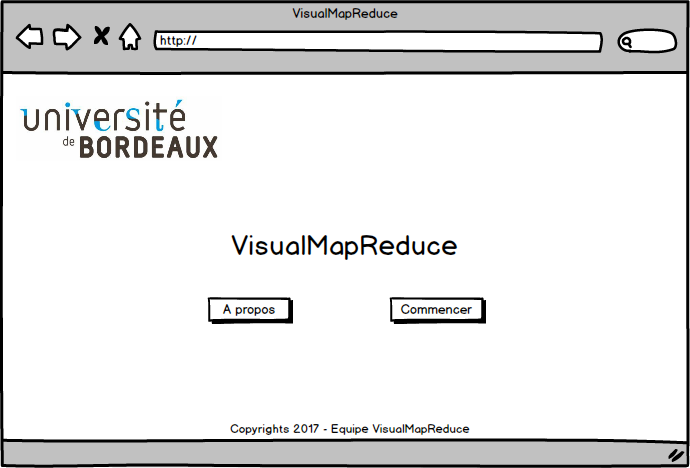
\includegraphics[width=0.75\textwidth]{images/interface/page_accueil.png}
    \caption{Page d'accueil}
\end{figure}

\begin{figure}[H]
  \centering
    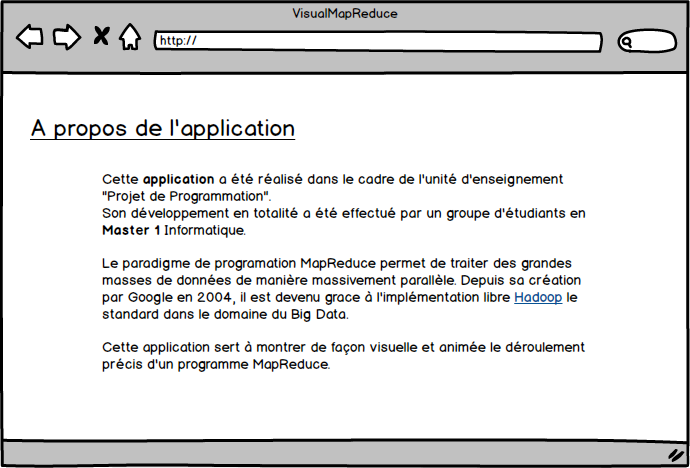
\includegraphics[width=0.75\textwidth]{images/interface/page_a_propos.png}
    \caption{A propos}
\end{figure}

\begin{figure}[H]
  \centering
    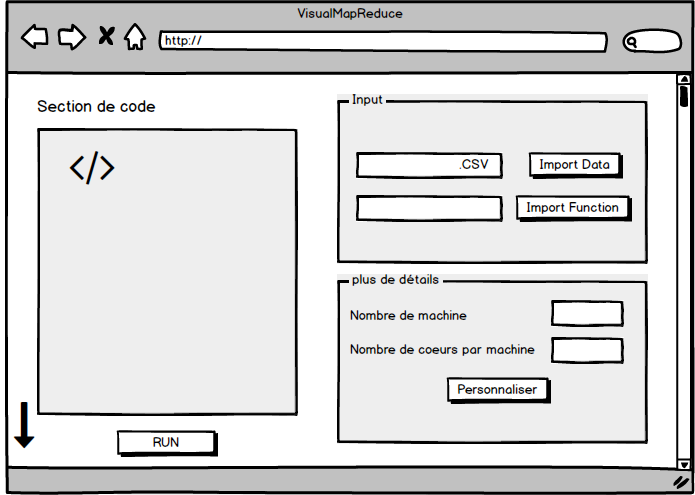
\includegraphics[width=0.75\textwidth]{images/interface/page_interpret1.png}
    \caption{Page d'interprétation}
\end{figure}

\begin{figure}[H]
  \centering
    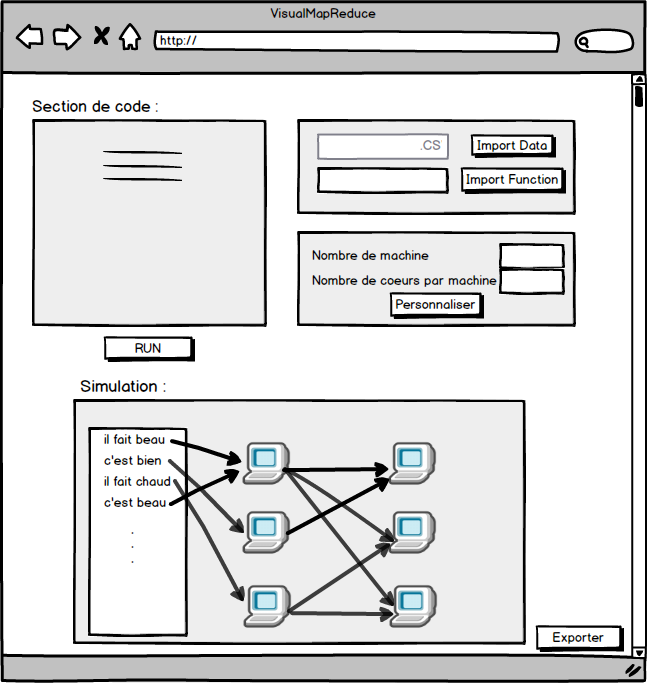
\includegraphics[width=0.75\textwidth]{images/interface/page_interpret2.png}
    \caption{Affichage du résultat}
\end{figure}

L'application étant monopage, le résultat de la simulation est directement affichée sur la même page où l'utilisateur remplit les données. Le graphique apparaît en dessous de la première section.

\begin{figure}[H]
  \centering
    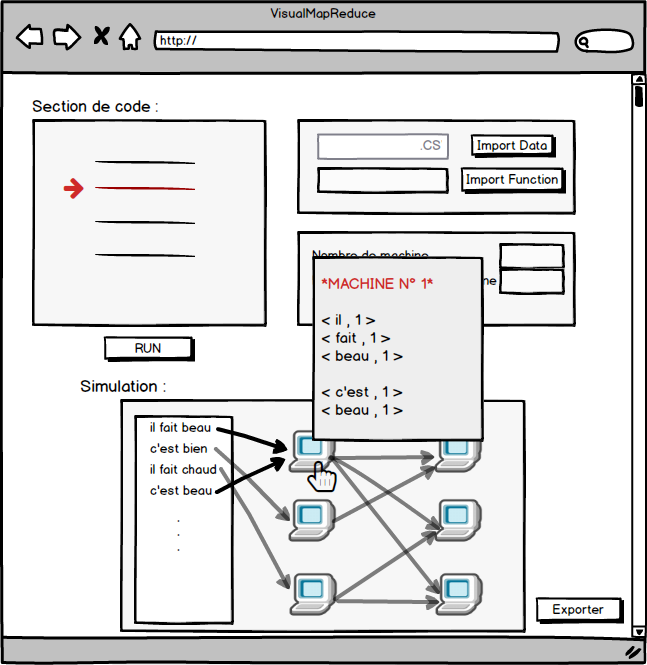
\includegraphics[width=0.75\textwidth]{images/interface/page_interpret3.png}
    \caption{Détail d'une machine}
\end{figure}

Comme illustré dans la figure ci-dessus, l'utilisateur a la possibilité de consulter les détails d'exécution qui concernent une machine particulière. Lorsque l'utilisateur appuie sur l'icône de l'une des machines, l'ensemble des propriétés qui concernent celle-ci s'affichent à l'écran. Au début du projet, ce besoin n'était pas très clair et nous avons cru comprendre qu'il peut aussi voir quelle partie de la section de code est exécutée sur cette machine. Or, nous nous sommes rendu compte plus tard que ce qu'il peut consulter c'est les données traitées sur chaque slot exécutant une des phases map ou reduce.